\documentclass[12pt,a4paper]{article}

% ─── 1. PACKAGES ──────────────────────────────────────────────────────────────
\usepackage[utf8]{inputenc}
\usepackage[T1]{fontenc}
\usepackage{amsmath, amssymb}
\usepackage{geometry}
\usepackage{graphicx}
\usepackage{xcolor}
\usepackage{listings}
\usepackage{hyperref}
\usepackage{booktabs}
\usepackage{enumitem}
\usepackage{tcolorbox}
\usepackage{mdframed}
\usepackage{fancyhdr}
\usepackage{titlesec}
\usepackage{tikz} 
\usetikzlibrary{shapes.geometric, positioning, arrows.meta, calc, trees}

% Font Settings
\usepackage{newtxtext,newtxmath} % Times New Roman
\usepackage{courier}             % Courier New untuk kode

\geometry{margin=2.5cm}

% ─── 2. WARNA TEMA ────────────────────────────────────────────────────────────
\definecolor{codebg}{RGB}{245,247,250}
\definecolor{codeframe}{RGB}{180,195,215}
\definecolor{keywordcolor}{RGB}{0,112,192}
\definecolor{commentcolor}{RGB}{100,160,100}
\definecolor{stringcolor}{RGB}{180,70,50}
\definecolor{notebg}{RGB}{255,249,230}
\definecolor{noteframe}{RGB}{230,180,50}
\definecolor{tipbg}{RGB}{230,245,235}
\definecolor{tipframe}{RGB}{50,160,90}
\definecolor{sectioncolor}{RGB}{30,80,150}

% ─── 3. STYLE SECTION & TOC ───────────────────────────────────────────────────
\titleformat{\section}{\Large\bfseries\color{sectioncolor}}{}{0em}{\thesection\quad}[\titlerule]
\titleformat{\subsection}{\large\bfseries\color{sectioncolor!80}}{}{0em}{\thesubsection\quad}

% Style Table of Contents
\usepackage{tocloft}
\renewcommand{\cftsecleader}{\cftdotfill{\cftdotsep}}
\renewcommand{\cftsecfont}{\bfseries\color{sectioncolor}}

% ─── 4. LISTINGS (CODE STYLE) ─────────────────────────────────────────────────
\lstdefinestyle{customstyle}{
  basicstyle=\ttfamily\small,
  backgroundcolor=\color{codebg},
  frame=single,
  rulecolor=\color{codeframe},
  keywordstyle=\bfseries\color{keywordcolor},
  commentstyle=\itshape\color{commentcolor},
  stringstyle=\color{stringcolor},
  numbers=left,
  numberstyle=\tiny\color{gray},
  breaklines=true,
  tabsize=4,
  showstringspaces=false
}
\lstset{style=customstyle}

% ─── 5. KOTAK CATATAN (MD-FRAME) ──────────────────────────────────────────────
\newmdenv[
  backgroundcolor=notebg, linecolor=noteframe, linewidth=2pt,
  leftline=true, topline=false, rightline=false, bottomline=false,
  innerleftmargin=10pt, innertopmargin=6pt, innerbottommargin=6pt, skipabove=8pt
]{notebox}

\newmdenv[
  backgroundcolor=tipbg, linecolor=tipframe, linewidth=2pt,
  leftline=true, topline=false, rightline=false, bottomline=false,
  innerleftmargin=10pt, innertopmargin=6pt, innerbottommargin=6pt, skipabove=8pt
]{tipbox}

% ─── 6. HEADER & FOOTER ───────────────────────────────────────────────────────
\pagestyle{fancy}
\fancyhf{}
\fancyhead[L]{\small\textit{Rekayasa Perangkat Lunak}}
\fancyhead[R]{\small\textit{noteify -- Analisis Kebutuhan}}
\fancyfoot[C]{\thepage}
\renewcommand{\headrulewidth}{0.4pt}

% ─── 7. DATA COVER ────────────────────────────────────────────────────────────
\title{
  {\LARGE\bfseries REKAYASA PERANGKAT LUNAK}\\[0.5em]
  {\large Modul Pembelajaran: Analisis Kebutuhan Perangkat Lunak}\\[0.8em]
  {\normalsize Penjelasan komprehensif mengenai rekayasa kebutuhan (requirements engineering), metode penggalian data, serta klasifikasi kebutuhan fungsional dan non-fungsional.}
}
\author{}
\date{}

% ==============================================================================
\begin{document}

\maketitle
\thispagestyle{fancy}
\tableofcontents
\newpage

% ─── KONTEN MATERI ─────────────────────────────────────────────────────────────

\section{Pemahaman Rekayasa Kebutuhan}

\subsection{Apa itu Rekayasa Kebutuhan?}
Dalam proses membangun sebuah perangkat lunak, tahap yang paling rawan dan menentukan kesuksesan proyek adalah tahap awal: \textbf{Rekayasa Kebutuhan} (\textit{Requirements Engineering}). 

Secara definisi, rekayasa kebutuhan adalah proses pembentukan layanan-layanan (fungsionalitas) yang dibutuhkan oleh \textit{customer} (pelanggan) dari sebuah perangkat lunak, beserta batasan-batasan (kendala teknis maupun operasional) di mana sistem tersebut nantinya beroperasi dan dikembangkan. 

Singkatnya, ini adalah proses "menerjemahkan bahasa keinginan pelanggan" menjadi "bahasa teknis" yang siap dieksekusi oleh tim pemrogram.

\subsection{Kenapa Kita Butuh Rekayasa Kebutuhan?}
Alasannya sangat sederhana dan mendasar: \textbf{karena kita membangun software untuk Customer (Pelanggan)}. 

\begin{notebox}
\textbf{Kutipan Head First:}\\
\textit{"If your customer is not happy with your software, that means you build a wrong software."} \\
(Jika pelangganmu tidak senang dengan perangkat lunakmu, itu berarti kamu telah membangun perangkat lunak yang salah.)
\end{notebox}

Penyebab paling umum kegagalan proyek \textit{software} adalah \textbf{Poor Communication} (Komunikasi yang buruk) antara tim pengembang dan pelanggan. Seringkali pelanggan meminta A, namun \textit{developer} menangkapnya sebagai B, dan akhirnya membangun sistem C. Oleh karena itu, seorang \textit{Software Engineer} yang baik dituntut \textbf{harus bisa menjadi pendengar yang baik} sekaligus \textbf{pemberi saran yang baik}. 

Namun perlu diingat, \textit{developer} juga harus hati-hati dengan apa yang disebut \textit{"Fool Customer"}—yaitu pelanggan yang sering kali tidak tahu persis apa yang mereka butuhkan atau permintaannya tidak masuk akal secara teknis. Di sinilah peran "pemberi saran yang baik" diuji.

\newpage
\section{Metode Penggalian Kebutuhan}

Lalu, bagaimana cara kita "merekayasa" atau menggali kebutuhan pelanggan tersebut? Walaupun masing-masing model proses SDLC (seperti Waterfall, Agile, atau Prototype) punya pendekatan tersendiri dalam rekayasa kebutuhan, namun tujuannya tetap sama: \textbf{mendapatkan daftar (\textit{list}) kebutuhan yang jelas pada perangkat lunak yang akan dibangun}.

Ada empat metode utama yang biasa digunakan untuk menggali kebutuhan (\textit{requirements elicitation}):

\begin{enumerate}
    \item \textbf{Wawancara (Interview):}
    Ini adalah komunikasi verbal langsung (tatap muka atau virtual) untuk mendapatkan informasi secara mendalam dari satu atau sekelompok orang (klien/pengguna akhir). 
    \item \textbf{Kuesioner (Questionnaire):}
    Komunikasi dalam bentuk pertanyaan tertulis yang disebarkan dan diberikan kepada \textit{customer}. Sangat cocok digunakan jika kita butuh data dari ratusan atau ribuan calon pengguna sekaligus secara masif.
    \item \textbf{Observasi (Observation):}
    Peninjauan secara langsung dan penilaian tentang apa yang sebenarnya terjadi pada suatu proses bisnis di lapangan. Kadang pelanggan tidak bisa menjelaskan cara kerjanya, jadi \textit{developer} harus melihat langsung ke lokasi.
    \item \textbf{Analisa Dokumen Manual:}
    Pencarian, pemahaman, dan pengkajian tentang dokumen-dokumen manual (kertas, form, laporan cetak) yang saat ini ada pada suatu kasus dan nantinya akan didigitalisasi ke dalam \textit{software}.
\end{enumerate}

\newpage
\section{Klasifikasi Tingkatan Kebutuhan}

Kebutuhan pada \textit{software} tidak bisa langsung ditulis dengan bahasa kode. Ia dimulai dari domain masalah bahasa manusia, yang kemudian dipecah menjadi bahasa teknis.

\subsection{1. User Requirement (Kebutuhan Pengguna)}
Dimulai dari domain masalah yang dikenal sebagai \textit{user requirement}. Ini adalah tentang \textbf{apa yang user harapkan untuk bisa dilakukan pada suatu perangkat lunak}. 
\begin{itemize}
    \item Biasanya dituliskan dalam bentuk \textit{User Requirement Document} atau bisa juga disampaikan secara kasual dalam bentuk \textit{user stories}.
    \item \textbf{Karakteristik:} Kedetailan informasinya tidak terlalu detail, target utamanya adalah pengguna sistem yang tidak mempunyai pengetahuan teknis yang dalam, dan bentuk informasinya berupa bahasa natural.
\end{itemize}

\subsection{2. System Requirement (Kebutuhan Sistem)}
Dari \textit{User Requirement}, daftar keinginan pelanggan tadi akan didetailkan ke dalam bentuk solusi domain yang dikenal sebagai \textit{System Requirement}. 
\begin{itemize}
    \item \textbf{Karakteristik:} Kedetailan informasinya sangat detail, target penggunanya adalah para \textit{Developer} (pengembang), dan bentuk informasinya bisa berupa grafik, bahasa teknis, format kode, tabel kebutuhan, atau diagram teknis.
\end{itemize}

\begin{notebox}
\textbf{Contoh Pemetaan:}
\begin{itemize}
    \item \textbf{User Requirement:} "Petugas perpustakaan harus bisa menambahkan data buku ke dalam sistem sesuai aturan".
    \item \textbf{System Requirement Specification:}
    \begin{itemize}
        \item Data buku yang disimpan antara lain: kode ISBN, judul buku, penerbit, pengarang.
        \item ISBN harus diisi dengan format: \texttt{xxx-999-xxx-999}.
        \item Tidak boleh ada data yang dikosongkan pada form data buku.
        \item Untuk mengisi data pengarang, petugas perpustakaan memilih dari data pengarang yang sudah ada di \textit{database}.
        \item Sistem bisa melakukan pengisian data buku secara otomatis dengan \textit{crawling}/mengambil data API dari \texttt{amazon.com}.
    \end{itemize}
\end{itemize}
\end{notebox}

\newpage
\section{Kebutuhan Fungsional vs Non-Fungsional}

Apapun level dokumennya (User maupun System Requirement), \textbf{sebuah kebutuhan yang baik harus terukur dan dapat diuji}. Kebutuhan ini secara fundamental dibagi menjadi dua tipe besar: Fungsional dan Non-Fungsional.

\subsection{Kebutuhan Fungsional (Functional Requirement)}
Kebutuhan fungsional adalah \textbf{pernyataan dari layanan (fitur) sistem yang harus disediakan}. Ini menjelaskan bagaimana sistem harus bereaksi terhadap \textit{input} tertentu, dan bagaimana sistem harus berperilaku dalam situasi tertentu. Intinya: apa yang \textit{software} \textbf{harus bisa lakukan}.

\textbf{Contoh Kebutuhan Fungsional:}
\begin{itemize}
    \item Pengguna bisa menambahkan komentar pada status yang muncul di \textit{timeline}.
    \item Sistem menyediakan filter foto "Clarendon" yang bisa dipilih pengguna.
    \item Pengguna bisa me-\textit{mention} (menyebutkan) teman pada \textit{tweet} yang dibuat.
    \item Mahasiswa bisa memilih kelas KRS sesuai dengan pilihan kelas yang disediakan.
\end{itemize}

\subsection{Kebutuhan Non-Fungsional (Non-Functional Requirement)}
Kebutuhan non-fungsional adalah \textbf{batasan-batasan} dari layanan-layanan (fungsional) sebuah sistem. Walaupun bernama "non-fungsional", kebutuhan ini \textbf{tetap wajib dipenuhi} agar aplikasi bisa beroperasi dengan baik di dunia nyata. Ini meliputi batasan waktu respon, batasan kapasitas, serta batasan-batasan dari \textit{environment} pengguna. Intinya: bagaimana \textit{software} harus \textbf{berperforma} dan \textbf{merespon keadaan}.

Kebutuhan non-fungsional seringkali dinyatakan oleh pelanggan secara tidak terukur (mengambang). Tugas \textit{Software Engineer} adalah merubahnya menjadi ukuran yang pasti.

\begin{table}[h]
\centering
\begin{tabular}{@{}p{6.5cm}p{7.5cm}@{}}
\toprule
\textbf{Contoh Pernyataan Pelanggan (Tidak Terukur)} & \textbf{Spesifikasi Kebutuhan Terukur (Developer)} \\ \midrule
"Sistem yang dibangun harus \textit{user-friendly}" & "Antarmuka yang dibangun harus berbentuk \textit{menu-driven}, dan menggunakan komponen UI yang tepat seperti \textit{radio button}, \textit{check box}, dll." \\ \addlinespace
"Semua tampilan harus muncul dengan cepat di layar" & "Ketika user mengakses tampilan, halaman akan ter-\textit{render} muncul di layar dalam waktu kurang dari 3 detik" \\ \addlinespace
"Usaha untuk login harus dibatasi agar aman" & "Seorang user hanya mendapatkan kesempatan maksimal 3 kali salah memasukkan \textit{password} login pada sistem" \\ \bottomrule
\end{tabular}
\caption{Konversi Pernyataan Non-Fungsional Menjadi Terukur}
\end{table}

\newpage
\section{Klasifikasi Mendalam Kebutuhan Non-Fungsional}

Kebutuhan non-fungsional memiliki hirarki cabang yang sangat luas. Secara umum terbagi menjadi tiga kategori besar: \textbf{Product Requirement}, \textbf{Organizational Requirement}, dan \textbf{External Requirement}.

\begin{figure}[h]
    \centering
    \resizebox{\textwidth}{!}{
    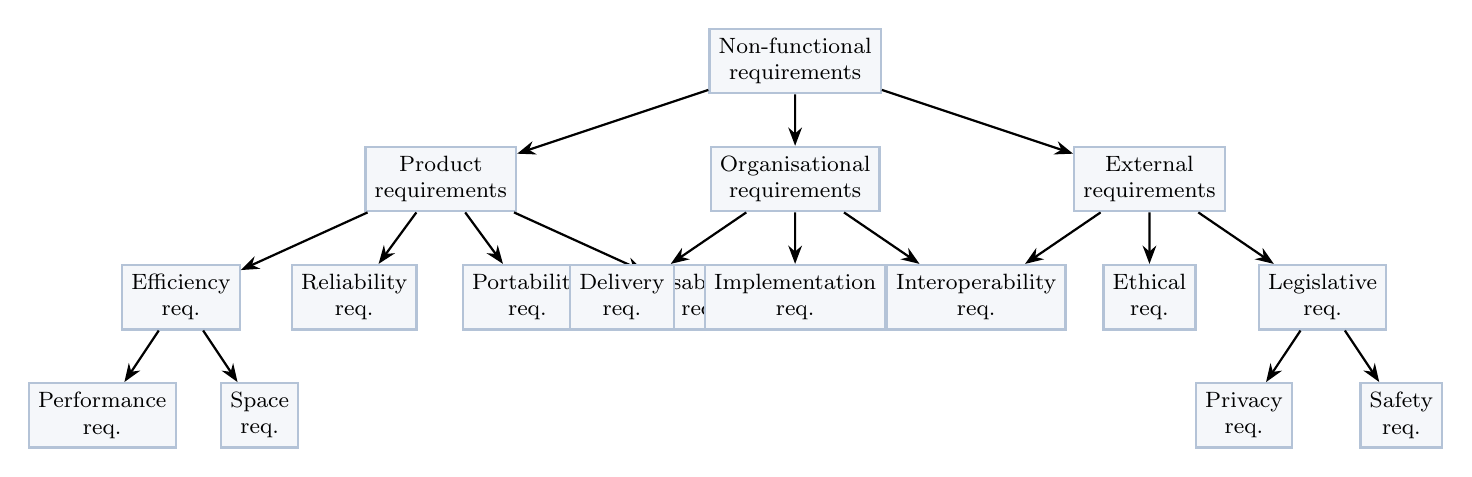
\begin{tikzpicture}[
        basic/.style={draw, rectangle, minimum height=0.6cm, align=center, fill=codebg, draw=codeframe, thick, font=\footnotesize},
        edge from parent/.style={draw, thick, -{Stealth[scale=1]}},
        level 1/.style={sibling distance=4.5cm, level distance=1.5cm},
        level 2/.style={sibling distance=2.2cm, level distance=1.5cm},
        level 3/.style={sibling distance=2cm, level distance=1.5cm}
    ]

    \node[basic] {Non-functional\\requirements \textnormal{}}
        child {node[basic] {Product\\requirements \textnormal{}}
            child {node[basic] {Efficiency\\req. \textnormal{}}
                child {node[basic] {Performance\\req. \textnormal{}}}
                child {node[basic] {Space\\req. \textnormal{}}}
            }
            child {node[basic] {Reliability\\req. \textnormal{}}}
            child {node[basic] {Portability\\req. \textnormal{}}}
            child {node[basic] {Usability\\req. \textnormal{}}}
        }
        child {node[basic] {Organisational\\requirements \textnormal{}}
            child {node[basic] {Delivery\\req. \textnormal{}}}
            child {node[basic] {Implementation\\req. \textnormal{}}}
            child {node[basic] {Standards\\req. \textnormal{}}}
        }
        child {node[basic] {External\\requirements \textnormal{}}
            child {node[basic] {Interoperability\\req. \textnormal{}}}
            child {node[basic] {Ethical\\req. \textnormal{}}}
            child {node[basic] {Legislative\\req. \textnormal{}}
                child {node[basic] {Privacy\\req. \textnormal{}}}
                child {node[basic] {Safety\\req. \textnormal{}}}
            }
        };
    \end{tikzpicture}
    }
    \caption{Hirarki Klasifikasi Kebutuhan Non-Fungsional.}
\end{figure}

Berikut adalah beberapa parameter properti yang biasa dijadikan acuan agar kebutuhan non-fungsional produk (Product Requirement) menjadi valid dan terukur:
\begin{itemize}
    \item \textbf{Kecepatan (Performance):} Diukur dengan besaran transaksi yang diproses per detik, waktu respon terhadap perintah pengguna (waktu layanan $< 2$ sekon), atau waktu \textit{refresh} layar.
    \item \textbf{Ukuran (Space):} Diukur dalam satuan K Bytes, atau jumlah konsumsi minimum RAM. Misal: Penyimpanan harus hemat, ukuran file unggahan $< 10$ MB.
    \item \textbf{Kemudahan Penggunaan (Usability):} Diukur dari waktu pelatihan staf untuk menguasai sistem, atau jumlah menu \textit{Help} (bantuan) yang disediakan.
    \item \textbf{Reliabilitas (Keandalan):} Diukur berdasarkan rata-rata waktu terjadinya kegagalan (\textit{Mean Time to Failure}), probabilitas sistem tidak bisa diakses, jumlah kegagalan, dan \textit{Availability} (ketersediaan server $99.9\%$).
    \item \textbf{Robustness (Ketahanan):} Diukur dari waktu yang dibutuhkan untuk \textit{restart/recovery} ketika terjadi \textit{crash}, persentase kegagalan \textit{event}, dan probabilitas hilangnya data (\textit{data loss}) akibat \textit{crash}.
    \item \textbf{Portability:} Diukur dari persentase kode (statement) yang berhasil dieksekusi lintas \textit{platform} OS. Misal: "Sistem harus bisa berjalan di Windows dan Linux tanpa modifikasi".
\end{itemize}

\end{document}